% !TeX root = disseration.tex
\chapter{IoT technology and IoT Acceptance}\label{chapter:Relatedwork1}
In this chapter, we first discuss how Internet-of-Things enter into people's daily lives, how people benefit from using IoT, what kinds of disadvantages IoT has brought, and the aspects that current IoT research has focused on. We then look at what factors are affecting potential IoT users when they are considering \textit{adopting} this new technology.

When users are considering adopting new IoT devices, they want to take the benefits of using IoT devices by sharing and disclosing certain personal information to get a more personalized experience~\cite{hemant2015internet}. However, such disclosed information could be accessed by other smart devices owned by themselves, other people, organizations, the government, or some third-parties with good or bad purpose, which brings privacy risks to the users~\cite{medaglia2010overview}. Thus, we attempt to obtain a clear understanding of the IoT acceptance model before our further research for the following reasons: 1) The factors that affect users' adopting phase may have a high chance to also have an effect on users' real using phase, which could help us understand how the IoT users make privacy decisions when they share their personal data in different IoT contexts; 2) These factors may further affect how we design the user interface for setting privacy preferences and recommend privacy-settings for different IoT contexts; 3) These factors can potentially help us develop the scales to evaluate the interfaces that we design, and build a theoretical model.

\section{IoT Technology}
The term ``Internet of Things" (IoT) was first introduced by Kevin Ashton in the context of supply chain management in 1999~\cite{ashton2009internet}. Atozri et al. define IoT as a pervasive presence around us of a variety of things or objects - such as Radio-Frequency IDentification (RFID) tags, sensors, actuators, mobile phones, etc. -- which, through a unique addressing scheme, are able to interact with each other and cooperate with their neighbors to reach common goals~\cite{atzori2010internet}. As various wireless sensor technologies (e.g. RFID, embedded sensors, and actuator nodes) and artificial intelligence have advanced rapidly during the last two decades, the definition of IoT has evolved to more broadly covering a wide range of monitoring and control applications based on a network of sensing and actuating devices that are controlled remotely through the Internet in many fields, such as tracking, transportation, household usage, healthcare and fitness~\cite{li2011smart, solima2016object, kelly2013towards, jia2012rfid, hassanalieragh2015health}.

IoT can benefit both organizations and individual consumers in all above-mentioned domains by enhancing data collection, enabling real-time response, improving access and control of internet-connected devices, increasing efficiency, productivity, and satisfaction~\cite{weinberg2015internet, porter2014smart}. With such huge social and economic potential, IoT is estimated to grow rapidly by a wide range of well-respected organizations. For example, Gartner~\cite{eddy2015gartner} has predicted over 21 billion IoT devices will be in use by 2020; IoT product and service suppliers will generate incremental revenue exceeding \$300 billion. IDC forecasts a global market for IoT will grow from \$1.9 trillion in 2013 to \$7.1 trillion in 2020. However, there exist several key security and privacy concerns associated with the rise of the IoT, including data processing and storage, privacy and security breaches\cite{weinberg2015internet, lu2014overview, yu2015handling}.

Previous studies mostly focused on the technical issues of IoT technologies~\cite{fantana2013iot, lazarescu2013design, shang2012internet}. For example, Uckelmann et al. systematically explained the architecture of future IoT~\cite{uckelmann2011architectural}. Chen et al. present a vision of IoT's applications in China~\cite{chen2014vision}. Guinard et al. described the IoT’s best practices based on the web technologies and proposed several prototypes using the web principles, which connect environmental sensor nodes, energy monitoring systems, and RFID-tagged objects to the web~\cite{guinard2011internet}. However, little attention has been devoted to, from the perspective of individual consumers, understanding how the user of IoT will trade off the above mentioned benefits and privacy concerns of IoT technology when they consider adopting it~\cite{al2016modeling, gao2014unified, mital2018adoption}.

Furthermore, researchers identified security and privacy issues as the major challenges for consumer acceptance of the IoT technology’s user-oriented IoT applications~\cite{medaglia2010overview}. Arguably, if the users find that their privacy demands can not be satisfied when using IoT devices after adopting them, they would probably finally give up using these devices.

\section{Model the Acceptance of IoT}
In this section, we first discuss the original Technology Acceptance Model and the adapted Unified Theory of Acceptance and Use of Technology (UTAUT) model. Then we look at what are the factors that affect potential IoT users to adopt IoT systems. 

\subsection{Technology Acceptance Model}
The Technology Acceptance Model (TAM) is arguably the most popular model that explains how users come to accept and use a technology~\cite{davis1989user}. TAM suggests that an individual's \textit{Behavioral Intention} to Use an information technology is significantly dependent upon the individual's \textit{Perceived Usefulness} and \textit{Perceived Ease Of Use} of that information technology. Specifically, perceived usefulness is the extent to which an individual believes that using a particular information technology will have a positive impact on his/her performance. Perceived ease of use is the extent to which an individual perceives that using a particular information technology will be free of effort. TAM also proposes that perceived ease of use can explain the variance in perceived usefulness.
TAM has been applied to a wide range of technology adoption contexts~\cite{wixom2005theoretical}, such as the adoption of PC~\cite{venkatesh2001longitudinal}, smartphones~\cite{park2007acceptance}, mobile marketing~\cite{bauer2005driving}, Internet banking~\cite{pikkarainen2004consumer}, facebook~\cite{lee2012effect, rauniar2014technology}, and online shopping~\cite{gefen2003trust}.

\subsection{UTAUT}
The unified theory of acceptance and use of technology (UTAUT) is a technology acceptance model proposed by Venkatesh et al.~\cite{venkatesh2003user}. Compared to TAM, UTAUT identifies four key factors: 1) performance expectancy, 2) effort expectancy, 3) social influence, and 4) facilitating conditions, related to predicting behavioral intention to use a technology and actual technology use primarily in organizational contexts. The first three factors are theorized and found to influence behavioral intention to use a technology, while behavioral intention and facilitating conditions determine technology use. UTAUT also identifies four moderators (i.e., age, gender, experience, and voluntariness).

UTAUT has been applied or extended in many contexts, such as electronic learning~\cite{wang2009interactive}, e-government~\cite{weerakkody2013examining}, and cloud computing~\cite{lian2015critical}. UTAUT is developed upon previous models of technology adoption, and designed specifically to investigate users’ acceptance of a new technology. Thus, it has explanatory power higher than previous models.

\subsection{The Acceptance of IoT}
Researchers have attempted to identify the factors that affect the acceptance of IoT by customers. Acquity Group~\cite{acquity2014internet} conducted a user study investigating the concerns of customers to adopt the IoT. Based on more than 2000 US-based customer survey, They find that awareness of the technology, usefulness, price (cost), security, privacy are the main concerns of the customers. In~\cite{gao2014unified}, Gao and Bai present a user study (N=368) to investigate the factors that affect the acceptance of IoT in China. They used the factors of TAM (i.e. perceived ease of use and perceived usefulness) along with other factors such as trust, social influence, perceived enjoyment, and perceived behavioral control. Their results show that perceived usefulness, perceived ease of use, social influence, perceived enjoyment, and perceived behavioral control have significant effect on users' behavioral intention to use the IoT. In~\cite{lee2019empirical}, Lee and Shin develop and test factors determining user acceptance of IoT services by extending current UTAUT model to include an extra hindering condition to explain the dual attitudes of users such as technical anxiety.

\subsection{A preliminary study (original work)}
We also conducted a preliminary/pilot study on Clemson University campus (N=15) with the aim to investigate the various factors that affect the adoption of IoT by interviewing with potential IoT users. The interviews were approximately 30-50 minutes in length and covered a wide range of open questions related to IoT. These questions asked participants about their personal preferences regarding to the technology and self-perceived tech savviness. In this study, the conversations with our participants were recorded only after obtaining their consent. This study was approved by IRB. The entire recorded conversation was then transcribed manually. We then extracted keywords from participants' statements during the interview, such as ``privacy'' or ``ease of use''. These keywords were then grouped using card sorting and affinity diagram techniques. We then used a grounded approach to creating a theory, which is shown in Figure~\ref{fig:pilotstudymodel}.

\begin{figure}
	\centering
	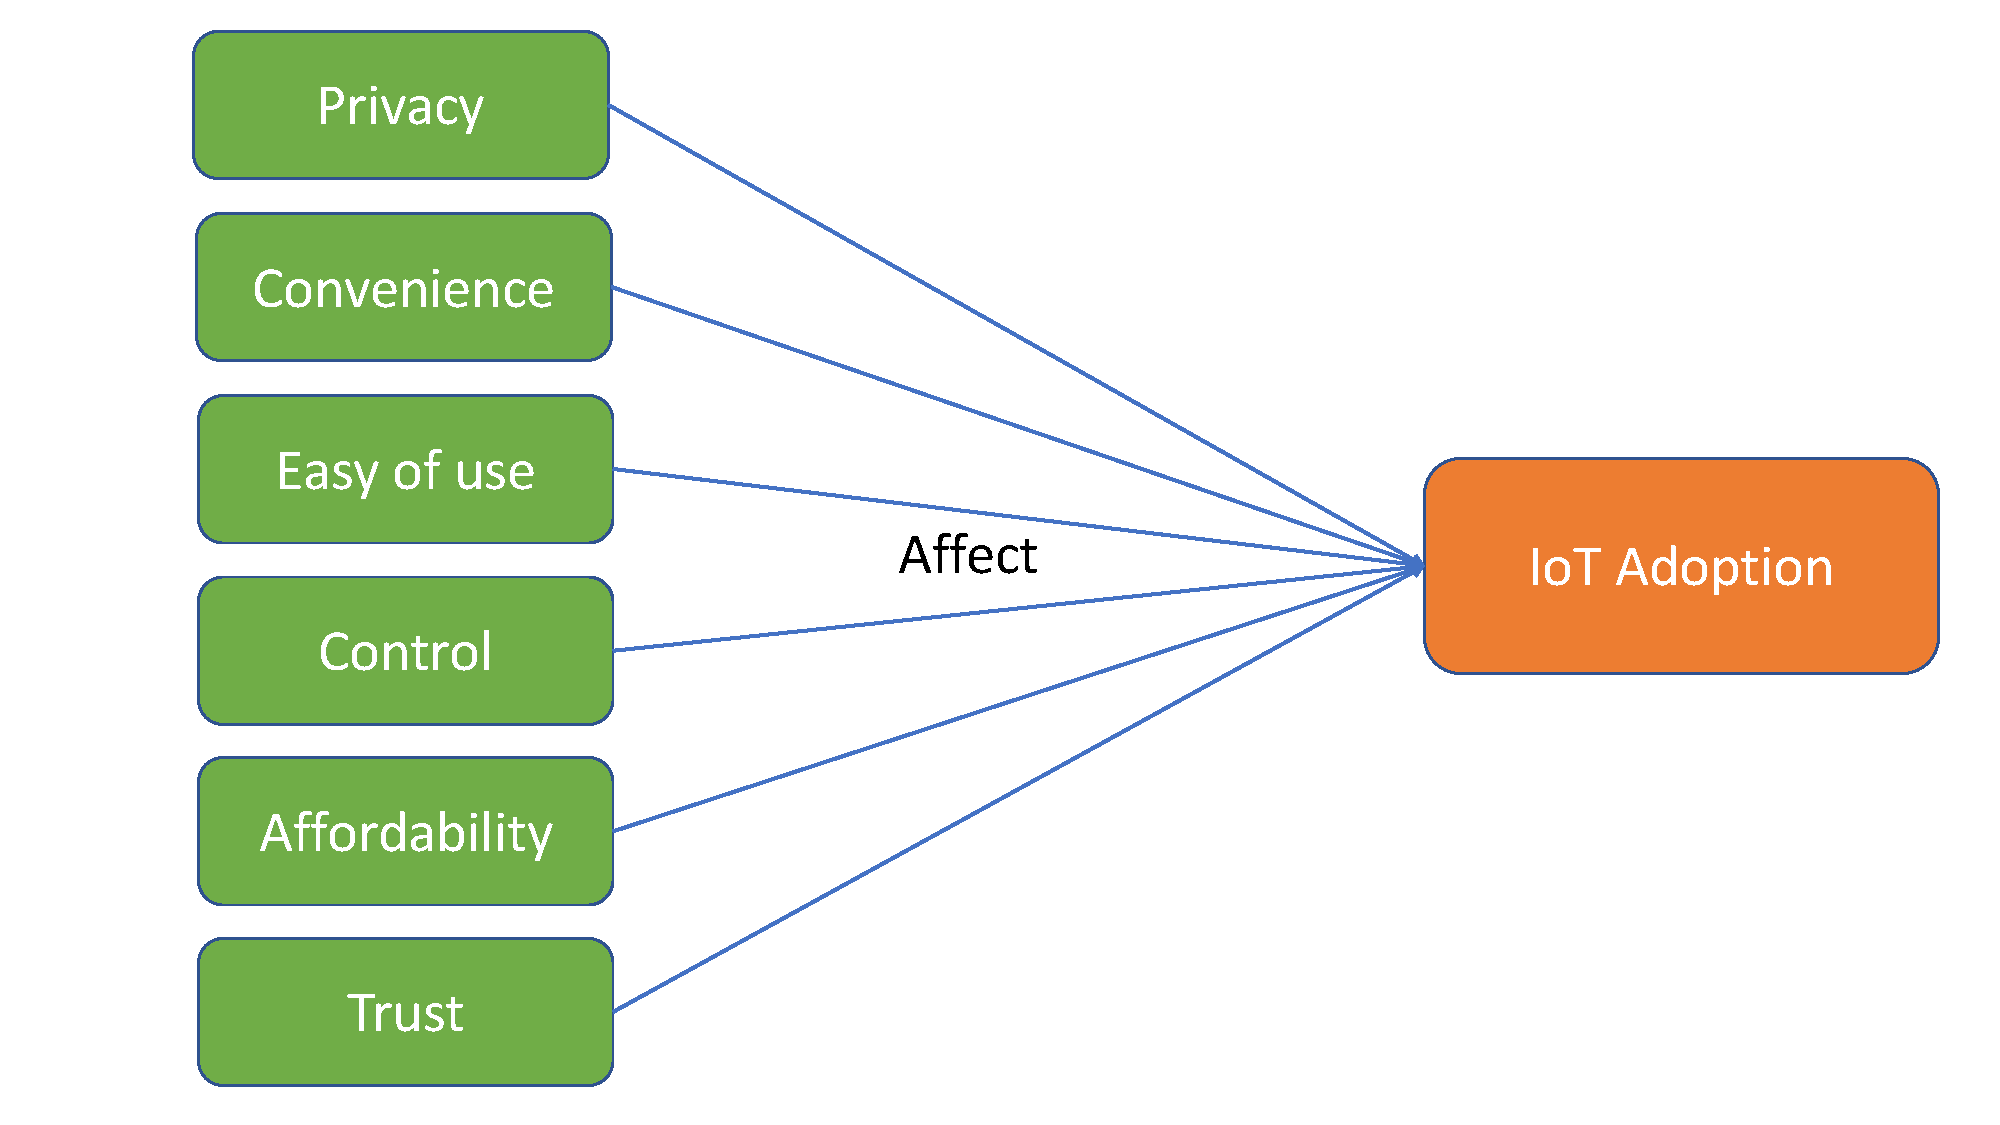
\includegraphics[width=0.8\textwidth]{figures/pilot_study_model.pdf}
	\caption{The factors that affecting users' adoptions of IoT found in our study}
	\label{fig:pilotstudymodel}
\end{figure}

The results showed similar findings as aforementioned work~\cite{gao2014unified, al2016modeling}. However, in our study, we noticed an interesting phenomenon that no literature has mentioned -- once trust with the manufacturers is established, it can propagate from the manufacturers to a third-party, which users are not aware of or even know about in the first place. We define this phenomenon as \textbf{Trust Chain}. An example of Trust Chain from our interview is:

\textit{I: ``Would you be alright if the manufacturer of those products collect your data and share with other organizations and provide more specific recommendation to you? Will you be OK with that?''}

\textit{P: ``I think I can be OK with that. Because the data this company collected are most time just shared or transferred to other companies who can analyze these data and get some information from these data.''}

\textit{I: ``Any company or any organization?''}

\textit{P: ``I think most are the manufacturers that I trust.''}

\textit{I: ``So you are OK with them to share your data?''}

\textit{P: ``Yes, I trust them.''}

As shown in Figure~\ref{fig:trustchain}, Trust Chain is established mostly because of the trust from the users to the manufacturers (i.e. the brand of the devices), and can arguably be categorized as an emotional behavior because users would not have a clear sight at the benefits and risks when they choose to trust the third parties that manufacturers choose to shared their data with. Such benefits and risks have been defined as abstract benefits and risk. One of our current undergoing research has shown that, in IoT domain, users are more likely to perceive concrete benefits and abstract risks, resulting this emotional behavior phenomenon. Such behavior could bring harm to their privacy and security. To be more rational, we suggest users to investigate the third parties that will handle their personal data. Thus, we suggest the manufacturer/designers of the IoT privacy to provide users transparency and control on what third parties they will share users' data with to reduce the risks of insecure Trust Chain sharing behavior.

\begin{figure}
	\centering
	
\includegraphics[width=0.75\columnwidth]{figures/trustchain.pdf}
	\caption{Trust Chain}
	\label{fig:trustchain}
\end{figure}

Knowing all these factors that affect users' decision on adopting IoT device will help us develop the scales for evaluating our designed privacy-setting interfaces in our proposed work (Chapter~\ref{chapter:evaluation}). Based on the insights gained from this study, we encourage the designers of IoT privacy-setting interfaces to face the difficult challenge of maximizing the usability and the privacy control of the user interface while minimizing the privacy threats to the users, making IoT more acceptable.

\section{Summary}
In this chapter, I have noted the following points: 1) IoT have grown in use rapidly with the advancing of RFID and other wireless sensor technologies. 2) IoT have brought convenience and enjoyment to our daily lives. 3) Privacy concern is an important factor that affect users' decisions when adopting IoT. 4) The acceptance of IoT is still not systematically examined.


In the next chapter, we discuss the reason that cause the privacy issues in IoT, how effective existing privacy control schemes are, and the work that aims to help users protect their privacy more effectively.



















\chapter{Privacy setting technologies in IoT}\label{chapter:Relatedwork2}
In chapter~\ref{chapter:Relatedwork1}, we discuss the development of IoT and its acceptance model. As IoT systems gain popularity and bring privacy issues at the same time, it is urgent to study the cause of these privacy issues. By doing this, we can improve our design of IoT applications to protect IoT users' privacy, and make IoT more acceptable.

\section{Privacy Preference}
Researchers have attempted to examine users' privacy preferences in different areas, such as Social Networks and mobile applications. Research has shown people differ extensively in their privacy settings~\cite{olson2005study}, but can be clustered into groups~\cite{anthony2007privacy,knijnenburg2013dimensionality}. In~\cite{wisniewski2014profiling, knijnenburg2017privacy}, Facebook users are found to belong to one of 6 types of privacy profiles which range from Privacy Maximizers to Minimalists. In the health/fitness domain, emerging sensors and mobile applications allow people to easily capture fine-grained personal data related to long term fitness goals. Brar and Kay discover that users' preferences change for every fitness/heath index. Weight was found the be the most important index~\cite{brar2004privacy}. 

At the same time, users are found to have difficulties managing their privacy settings with current privacy-setting schemes. Liu et al. use an online survey (N=200) to investigate the difference between the desired privacy settings and the actual privacy settings of Facebook users. Their results show that 63\% of the privacy settings for photo sharing did not match the users' desired settings. In~\cite{madejski2012study}, Madejski et al. conduct user studies to find the difference between Facebook users’ sharing intentions and their actual privacy settings. Their results show that there is at least one violation in the privacy settings for each of the 65 participants.

The reasons for the failure of existing privacy-setting schemes are diverse. One reason for this is that the increasing number of privacy rules make manual privacy configuration excessively challenging for normal users~\cite{furnell2015managing}. Knijnenburg et al. discover that people's information disclosure behaviors vary along multiple dimensions~\cite{knijnenburg2013dimensionality}. People can be classified along these dimensions into groups with different ``disclosure styles". This result suggests that we could classify users into their respective privacy groups and adapt their privacy practices to the disclosure style of this group to satisfy different types of information and users. However, on the other hand, the more privacy policies would lead to more decision-making and more burden for users. Note that in the IoT environment, the number for different IoT devices could be vast, which could potentially make choosing adequate privacy settings a very challenging task that is likely to result in information and choice overload~\cite{williams2016perfect}. Therefore, in this thesis, we will use a data-driven approach (machine learning techniques) to discover suitable smart privacy profiles, which are generated from the results of both statistical analysis and machine learning techniques, for users with different ``disclosure styles".

\section{Privacy in IoT}
IoT systems are capable of providing a highly personalized services to their users~\cite{vallee2016personalization, etzion2014personalization, hemant2015internet}. Henka et al.~\cite{henka2016personalizing} propose an approach to personalize services in household IoT using the Global Public Inclusive Infrastructure's~\cite{vanderheiden2011creating} preference set to describe an individual's needs and preferences, and then adapting a smart environment accordingly. Russell et al.~\cite{russell2015personalization} use unobtrusive sensors and a micro-controller to realize human detection to provide personalization in a household IoT environment.

Researchers have shown that privacy plays a limiting role in users' adoption of personalized services~\cite{teltzrow_2004}. For example, Awad and Krishnan~\cite{awad_2006} show that privacy concerns inhibit users' use of personalized services, and Sutanto et al.~\cite{sutanto_2013} demonstrated that privacy concerns can prevent people from using a potentially beneficial personalized application. Kobsa et al.~\cite{kobsa_2016} demonstrate that the personalization provider is an important determinant of users' privacy concerns.

Moreover, research has shown  users' willingness to provide personal information to personalized services depends on both the risks and benefits of disclosure~\cite{phelps_2000,ho_2006,hui_2006}, and researchers therefore claim that both the benefits and the risks meet a certain threshold~\cite{treiblmaier_2007}, or that they should be in balance~\cite{chellappa_2005}.

The argument that using user-generated data for personalization can result in privacy concerns has also been made in IoT environments~\cite{worthy_trust_2016, gao2014unified, al2016modeling}. One of the first examples in this regard was the work by Sheng et al.~\cite{sheng_experimental_2008}, who showed that users of ``u-commerce'' services (IoT-driven mobile shopping) felt less inclined to use personalized (rather than non-personalized) u-commerce services, unless the benefits were overwhelming (i.e., providing help in an emergency).

In response, researchers have proposed frameworks with guidelines for evaluating the security and privacy of consumer IoT applications, devices, and platforms~\cite{perera_privacy-by-design_2016, loi_systematically_2017}. Most of these guidelines are focused on minimizing data acquisition, storage, and collection sources. Along these guidelines, several researchers have proposed architectures that restrict unwanted access to users' data by IoT devices. For example, Davies et al. propose ``privacy mediators'' to the data distribution pipeline that would be responsible for data redaction and enforcement of privacy policies even before the data is released from the user's direct control~\cite{davies_privacy_2016}. Likewise, Jayraman et al.'s privacy preserving architecture aggregates requested data to preserve user privacy~\cite{jayaraman_privacy_2017}.

Other research has considered IoT privacy from the end-user perspective~\cite{feth_user-centered_2017}, both when it comes to research (e.g., Ur et al. investigated how privacy perceptions differ among teens and their parents in smart security systems installed in homes~\cite{ur_intruders_2014}) and design (e.g., Williams et al. highlight the importance of designing interfaces to manage privacy such that they are usable to the end users of IoT devices~\cite{williams2016perfect}, and Feth et al. investigated the creation of understandable and usable controls~\cite{feth_user-centered_2017}). We followed this approach and developed a novel data-driven approach to developing usable and efficient privacy-setting interfaces for several different IoT contexts.

\section{Existing Privacy Setting Models}
Previous studies in smartphone privacy have shown that the current smartphone privacy interfaces lack the potential to provide the necessary user privacy information or control for both Android and iOS systems~\cite{lin2014modeling}. Several solutions have been proposed to improve mobile privacy protection and offer users more privacy control~\cite{felt2012android, beresford2011mockdroid}. These lead into rapid improvement of privacy management of current mobile systems, providing more control on the user's privacy settings.

Android system mainly use Ask On Install (AOI) and Ask On First Use (AOFU) models for privacy settings~\cite{tsai2017turtle, wijesekera2017feasibility}. In the AOI model, the smartphone permissions are asked in bulk before installing a new app. The user's option is only to allow or deny all, which clearly gives less privacy control. Also, only few users would read or pay attention to the privacy settings when installing the app, and even fewer users can understand their meaning~\cite{felt2012android,kelley2012conundrum}. Several third-party apps have been developed to cope with this problem, such as Turtleguard~\cite{tsai2017turtle} and Mockdroid~\cite{beresford2011mockdroid}. %, Advanced Permission Manager\cite{},Xprivacy\cite{}, Permission Master~\cite{}, DonkeyGuard\cite{}, AppOps\cite{}. 
In the AOFU model~\cite{tsai2017turtle}, permissions are only asked during the first use of an app or when some function of the app is demanding a specific permission of the smartphone. In this case, the user will trade off his privacy (data sharing) and the functionality of the app. Users can also revisit and review permissions in their phone privacy settings for each app. This model makes users more informed and gives them more control compared to AOI~\cite{fu2014field}.

A few privacy management solutions were developed to simplify the task of controlling personal data for smartphone users. For instance, ipShield~\cite{chakraborty2014ipshield} is a context-aware privacy framework for mobile systems that provides users with great control of their data and inference risks. My Data Store \cite{ref:vescovi} offers a set of tools to manage, control and exploit personal data by enhancing an individual’s awareness of the value of their data. Similarly, Databox~\cite{ref:chaudhry} enables individuals to coordinate the collection of their personal data, and make those data available for specific purposes. However, these data managers do not include user privacy profiling and recommendation in the complex IoT environment. Privacy can also be protected by providing different anonymity levels of data that are given to third parties. However, it might not be possible to implement the most effective privacy standards such as data obfuscation due to numerous trade-offs and restrictions, especially in the health care and fitness domain.

In the smartphone domain, privacy nudging is an effective scheme to increase users' awareness~\cite{almuhimedi2015your}. Privacy nudging allows users to be informed about both their privacy settings and how third party applications access their data~\cite{liu2016follow,fu2014field}. In a study by Liu et al., 78.7\%~\cite{liu2016follow} of the nudges were adopted by smartphone users. However, such nudges are problematic for IoT, because IoT devices are supposed to operate in the background. Moreover, as the penetration of IoT devices in our homes continues to increase, nudging would become a constant noise which users would soon start to ignore, like software EULAs~\cite{good2005spyware} or privacy policies~\cite{jensen2004privacy}. In addition, privacy nudges lack the personalization and provide only a general recommendation.

%Another approach which is more user-centric is the user-tailored privacy~\cite{knijnenburg2017privacy}. It models users’ privacy concerns and provides them with adaptive privacy decision support. This model can be seen as personalized ``smart nudges'' where the recommendation is aligned with the user's privacy preference. User-tailored privacy aids users in making privacy decisions by providing them the right amount of both the privacy-related information associated to them and the useful privacy control that do not overwhelm or mislead them. However, in practice it is hard to implement general privacy model as the idea is too broad and abstract especially in the diversity of privacy perception of users. 

%\textit{khealth} is an IoT framework based on a personalized digital health care information system that protects users from third parties' advertisements~\cite{sharma2018toward}. Pejovic and Musolesi~\cite{Pejovic2014} presented the design and implementation of an efficient online learner that can serve as a basis for recognizing opportune moments for interruption. The design of the library is based on an in-depth study of human interruptibility. Comparatively, our work tries to find the most suitable privacy-setting profile for each user based on their privacy preference on different household IoT scenarios.

\section{Privacy-Setting Interfaces}
Beyond prompts, one can regulate privacy with global settings. The most basic privacy-setting interface is the traditional ``access control matrix'', which allows users to indicate which entity gets to access what type of information~\cite{sandhu1994access}. This approach can be further simplified by grouping recipients into relevant semantic categories, such as Google+'s \emph{circles}~\cite{watson12}. Taking a step further, Raber et al.~\cite{197908} proposed \emph{Privacy Wedges} to manipulate privacy settings. Privacy Wedges allow users to make privacy decisions using a combination of semantic categorization (the various wedges) and inter-personal distance (the position of a person on the wedge). Users can decide who gets to see various posts or personal information by ``coloring'' parts of each wedge. 

Privacy wedges have been tested on limited numbers of friends, and in the case of household IoT they are likely to be insufficient, due to the complexity of the decision space. To wit, IoT privacy decisions involve a large selection of devices, each with various sensors that collect data for a range of different purposes. This makes it complicated to design an interface that covers every possible setting~\cite{williams2016perfect}. A wedge-based interface will arguably not be able to succinctly represent such complexity, and therefore either be impossible, or still lead to a significant amount of information and choice overload. 

We used a data-driven approach to solve this problem: statistical analysis informs the construction of a layered settings interface, while machine learning-based privacy prediction helps us find smart privacy profiles.

\section{Privacy Prediction}
Several researchers have proposed privacy prediction as a solution to the privacy settings complexity problem---an approach known as ``user-tailored privacy'' (UTP)~\cite{knijnenburg2017}. Systems that implement UTP first predict users' privacy preferences and behaviors based on their known characteristics. They then use these predictions to provide automatic default settings or suggestions in line with users' disclosure profiles, to educate users about privacy features they are unaware of, to tailor the privacy-setting user interfaces to make it easier for users to engage with their preferred privacy management tools, or to selectively restrict the types of personalization a system is allowed engage in.

Most existing work in line with this approach has focused on providing automatic default settings. For example, Sadeh et al.~\cite{sadeh2009understanding} used a k-nearest neighbor algorithm and a random forest algorithm to predict users' privacy preferences in a location-sharing system, based on the type of recipient and the time and location of the request. They demonstrated that users had difficulties setting their privacy preferences, and that the applied machine learning techniques can help users to choose more accurate disclosure preferences. Similarly, Pallapa et al.~\cite{pallapa2014adaptive} present a system which can determine the required privacy level in new situations based on the history of interaction between users. Their system can efficiently deal with the rise of privacy concerns and help users in a pervasive system full of dynamic interactions.

Dong et al.~\cite{dong2016ppm} use a binary classification algorithms to give users personalized advice regarding their privacy decision-making practices on online social networks. They found that J48 decision trees provided the best results. Li and et al.~\cite{li2017cross} similarly use J48 to demonstrate that taking the user's cultural background into account when making privacy predictions improves the prediction accuracy. Our data stems from a culturally homogeneous population (U.S. Mechanical Turk workers), so cultural variables are outside the scope of our study. We do however follow these previous works in using J48 decision trees in our prediction approach.

We further extend this approach using \emph{clustering} to find several smart default policies (``profiles''). This is in line with Fang et al.~\cite{fang2010privacy}, who present an active learning algorithm that comes up with privacy profiles for users in real time. Since our approach is based on an existing dataset, our algorithm does not classify users in real time, but instead creates a static set of profiles `offline', from which users can subsequently choose. This avoids cold start problems, and does not rely on the availability of continuous real-time behaviors. This is beneficial for household IoT privacy settings, because users often specify their settings in these systems in a ``single shot'', leaving the settings interface alone afterwards.

Ravichandran et al.~\cite{ravichandran2009capturing} employ an approach similar to ours, using $k$-means clustering on users' contextualized location sharing decisions to come up with several default policies. They showed that a small number of policies could accurately reflect a large part of the location sharing preferences. 

In this proposal, we extend this \emph{clustering} approach to find the best profiles based on various novel clustering approaches, and take the additional step of designing user interfaces that incorporate the best solutions for different IoT contexts.

\section{Summary}
In this chapter, we have noted following points: 1) Existing research has shown that people are extensively different in their privacy settings, but can be grouped. 2) People are bad at managing privacy settings using currently privacy setting schemes. 3) Privacy prediction can be used by utilizing machine learning algorithms to help design a new privacy-setting interface to simplify the task of managing privacy setting for users. 

In the next chapter, we will present how we design for privacy in the general/public IoT context using a data-driven approach, the contributions and the limitations of our work.